\documentclass[11pt]{article}
\usepackage{listings}
\usepackage{graphicx}


%Gummi|065|=)
\title{\textbf{Project 2: Simulation of Gossip Protocol\\COP5615}}
\author{Rahul Prabhu\\
		Sanil Sinai Borkar}
\date{}
\begin{document}

\maketitle
\section{Description}

The following command was run at the command prompt:
\begin{lstlisting}
$ run <num_of_nodes> <topology> <algorithm>
\end{lstlisting}


There are 3 command-line arguments as given below:
\begin{enumerate}
\item \textbf{num\_of\_nodes}: The number of nodes in the network topology. It is a positive integer value.
\item \textbf{topology}: The network topology. It should be one of `full', `line', `3D' or `imp3D'.
\item \textbf{algorithm}: The algorithm. It should be either `gossip' (Gossip Protocol) or `push-sum' (Push-Sum Algorithm).
\end{enumerate}

For 3D and imperfect 3D topologies, we round it to the next highest cube of an integer. We tested our code on networks of sizes from 1000 to 1 million.

\section{Gossip Protocol}
We ran the gossip protocol on on all the four topologies with 1000 messages as the limit after which a node starts ignoring a gossip. Figure ~\ref{gossipresults} shows the results for all the simulations. 

\textit{The algorithm was run on all topologies several times and the times shown are averages over these runs.}

\begin{figure}[h]
    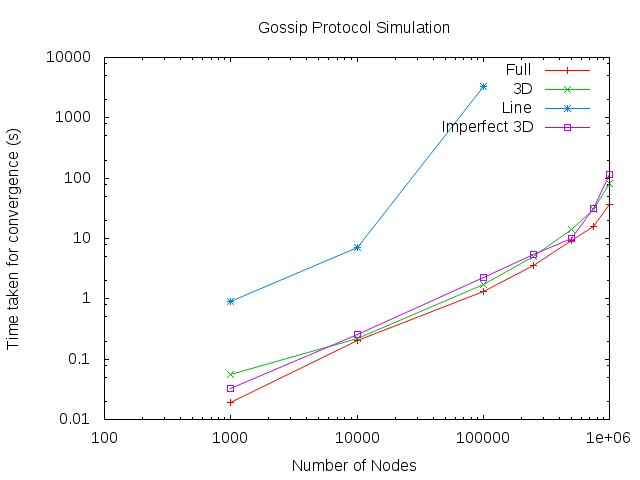
\includegraphics[scale=0.75]{Gossip.jpg}
    \caption{Gossip Protocol Run on various topologies of various sizes}
    \label{gossipresults}
\end{figure}


\section{Push-Sum Protocol}
We ran the push-sum protocol on on all the four topologies with $10^{-10}$ as the convergence value beyond which the nodes stop computation. Figure ~\ref{pushsumresults} shows the results for all the simulations. 

\textit{The algorithm was run on all topologies several times and the times shown are averages over these runs.}
\begin{figure}[h]
    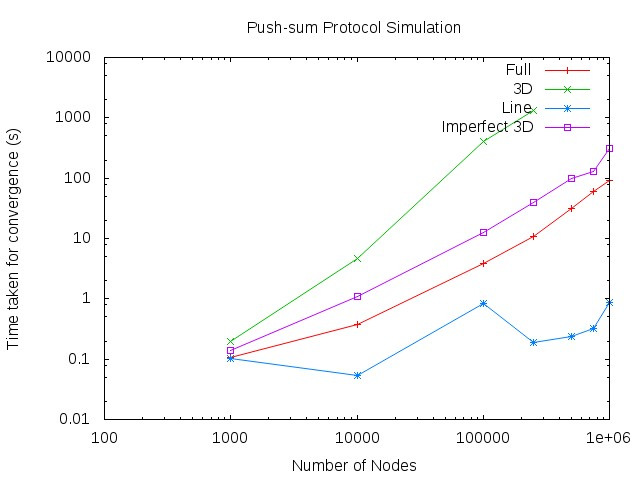
\includegraphics[scale=0.75]{pushsum.jpg}
    \caption{Push Sum Protocol Run on various topologies of various sizes}
    \label{pushsumresults}
\end{figure}



\section{Observations}
\subsection{Gossip Protocol}
For the gossip protocol a full topology takes the shortest time to converge since the number of hops a message has to make to reach the farthest node from the starting node is very small. 3D and imperfect 3D take longer than full to converge since a gossip has to navigate across the topology to make its way to the farthest node. For smaller number of nodes, we don't see too much difference in convergence time for 3D and imperfect 3D but as the number of nodes increase, imperfect 3D takes shorter times to converge. Line takes the longest to converge. This is intuitive since the number of hops a gossip has to make to reach the farthest node is very large. We did not run gossip on a line topology for sizes greater than 100,000 because it was taking too long to converge.

\subsection{Push-Sum Protocol}
The line topology takes the least amount of time to converge in the push-sum protocol. The behaviour seems erratic as the time to converge does not increase with the number of nodes. This starts making sense when we look at the actual average computed. Line topology gives the worst error among all the topologies. By error we mean the deviation of the computed average from the actual average value. This is because the number of nodes participating in the average computation before a convergence is reached is low. Among the three topologies that give very low error rates, full topology took the least time. Imperfect 3D took the next least amount of time followed by 3D. 3D was not run for topologies with number of nodes larger than 250,000.


\end{document}
